
\subsection*{3.1.}

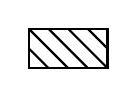
\begin{tikzpicture}
    % Clipper pour limiter les hachures à l'intérieur du rectangle
    \begin{scope}
        \clip (0,0) rectangle (1,0.5); % Définit la zone de découpe (rectangle)
        % Hachures inclinées
        \foreach \x in {-2,-1.75,...,6} {
            \draw[thick] (\x,0) -- (\x-0.5,0.5);}
    \end{scope}
    % Rectangle (bordure)
    \draw[thick] (0,0) rectangle (1,0.5);
\end{tikzpicture}
: aire correspondant à $\int_0^{15} P(t) \, dt = \dfrac{15 \times 500}{2} = 3750.$

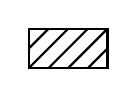
\begin{tikzpicture}
    % Clipper pour limiter les hachures à l'intérieur du rectangle
    \begin{scope}
        \clip (0,0) rectangle (1,0.5); % Définit la zone de découpe (rectangle)
        % Hachures inclinées (de bas à gauche vers haut à droite)
        \foreach \x in {-2,-1.75,...,6} {
            \draw[thick] (\x,0) -- (\x+0.5,0.5);}
    \end{scope}
    % Rectangle (bordure)
    \draw[thick] (0,0) rectangle (1,0.5);
\end{tikzpicture}
: aire correspondant à $\int_{15}^{t_f} P(t) \, dt = 500 \times (t_f - 15).$

\begin{center}
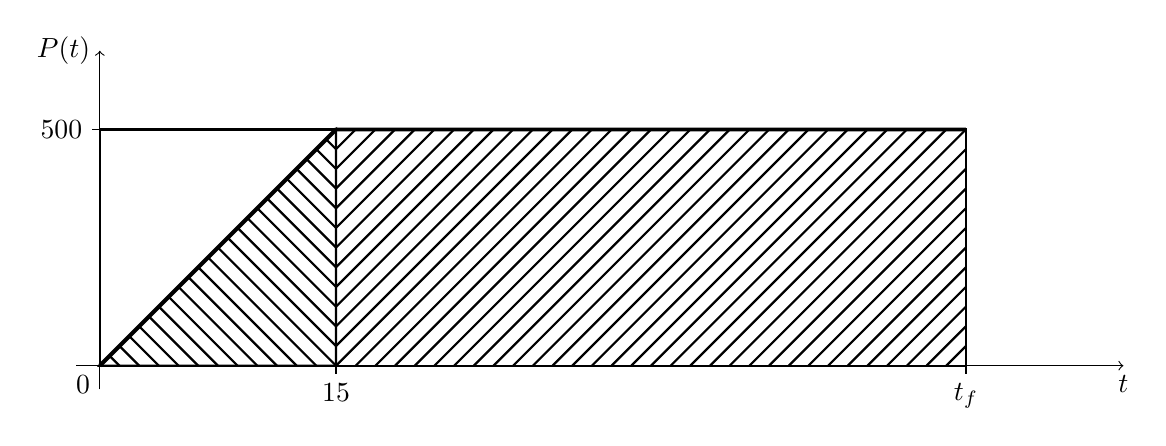
\begin{tikzpicture}
    % Axes
    \draw[->] (-0.3,0) -- (13,0) node[below] {$t$};
    \draw[->] (0,-0.3) -- (0,4) node[left] {$P(t)$};
    % Origine
    \node[below left] at (0,0) {0};
    % Graduations et labels
    \draw (0,3) -- (-0.1,3) node[left] {$500$};
    \draw (3,0) -- (3,-0.1) node[below] {$15$};
    \draw (11,0) -- (11,-0.1) node[below] {$t_f$};
    % Courbe
    \draw[line width=0.5mm] (0,0) -- (3,3) -- (11,3);
    % Clipper pour limiter les hachures à l'intérieur du rectangle
    \begin{scope}
        \clip (3,0) rectangle (11,3); % Définit la zone de découpe (rectangle)
        % Hachures inclinées (de bas à gauche vers haut à droite)
        \foreach \x in {-2,-1.75,...,13} {
            \draw[thick] (\x,0) -- (\x+3,3);}
    \end{scope}
    % Rectangle (bordure)
    \draw[thick] (0,0) rectangle (11,3);
    % Triangle rectangle isocèle
    \draw[thick] (0,0) -- (3,0) -- (3,3) -- cycle; % Dessin du triangle
    % Hachures inclinées
    \begin{scope}
        \clip (0,0) -- (3,0) -- (3,3) -- cycle; % Limiter les hachures au triangle
        \foreach \x in {0,0.25,...,8} {
            \draw[thick] (\x,0) -- (\x-3,3);}
    \end{scope}
\end{tikzpicture}
\end{center}

\subsection*{3.2.}
\[\int_{0}^{t_f} P(t) \, dt = \int_{0}^{15} P(t) \, dt + \int_{15}^{t_f} P(t) \, dt =  3750 + 500 \times (t_f - 15).\]

\subsection*{3.3.}
Sur $[0~;~15]$, $P$ est une fonction linéaire dont le coefficient directeur est :
$\dfrac{500 - 0}{15 - 0} = \dfrac{500}{15}.$

Ainsi : $P(t) = \dfrac{500}{15}t.$

Une primitive de $P(t)$ sur $\mathbb{R}$ est $\dfrac{1}{2}t^2 + C$ avec $C \in \mathbb{R}$ une constante.

Ainsi :
\begin{align*}
\int_{0}^{15} P(t) \, dt &= \int_{0}^{15} \frac{500}{15} t \, dt \\
&= \frac{500}{15} \times \int_{0}^{15} t \, dt \\
&= \frac{500}{15} \times \left[ \frac{1}{2}t^2 + C \right]_0^{15} \\
&= \frac{500}{15} \times \left( \frac{1}{2} \times 15^2 - \frac{1}{2} \times 0^2 \right) \\
&= \frac{500}{2} \times 15 \\
&= 3750
\end{align*}

\subsection*{4.}
On cherche donc $t_f$ tel que : $37000 = \int_{0}^{t_f} P(t) \, dt$

A la question \textbf{3.2.}, on a vu l'expression de l'intégrale en fonction de $t_f$, ce qui aboutit à :
\[37000 = 3750 + 500 \times (t_f - 15).\]

Soit :
\[33250 = 500 \times (t_f - 15) \iff t_f - 15 = \frac{33250}{500} = 66,5 \iff t_f = 81,5\]

Il faut \textbf{1 min 21 s} pour faire fondre la glace.

\subsection*{5.}
Le temps calculé à la question précédente est inférieur au temps réel de chauffe. Il faut donc remettre en question les hypothèses du calcul. On a fait l’hypothèse que l’ensemble de l’énergie fournie par le chauffage servait à faire fondre la glace. Expérimentalement, ce n’est pas réalisable car il est difficile de concentrer le chauffage uniquement sur la glace. 

Il y a forcément \textbf{une partie de l’énergie qui réchauffe l’air ambiant} (entre autre) alors que ce n’est pas souhaité. Cela explique qu’il faille plus de temps pour faire chauffer le glaçon.

\bigskip


